\subsection{Backend Design}\label{backend-design}
\subsubsection{Service API}\label{service-api}
Die API ist als Webservice aufgebaut welcher funktionale Requests beantworten kann. Es wird kein direkter Datenzugriff
\"uber CRUD Methoden zur Verf\"ugung gestellt. Die Business-Logik wird wenn m\"oglich vollst\"andig im Service
abgehandelt. So ist die Funktionalit\"at des ganzen Systems gekapselt und unabh\"angig von allenfalls in der Zukunft
weiteren entwickelten Clients.

Nachfolgend sind alle geplanten Service Methoden nach Controller gruppiert aufgelistet. Eine
interaktive Version ist unter \fullref{swagger} verlinkt.

\begin{figure}
  \centering
  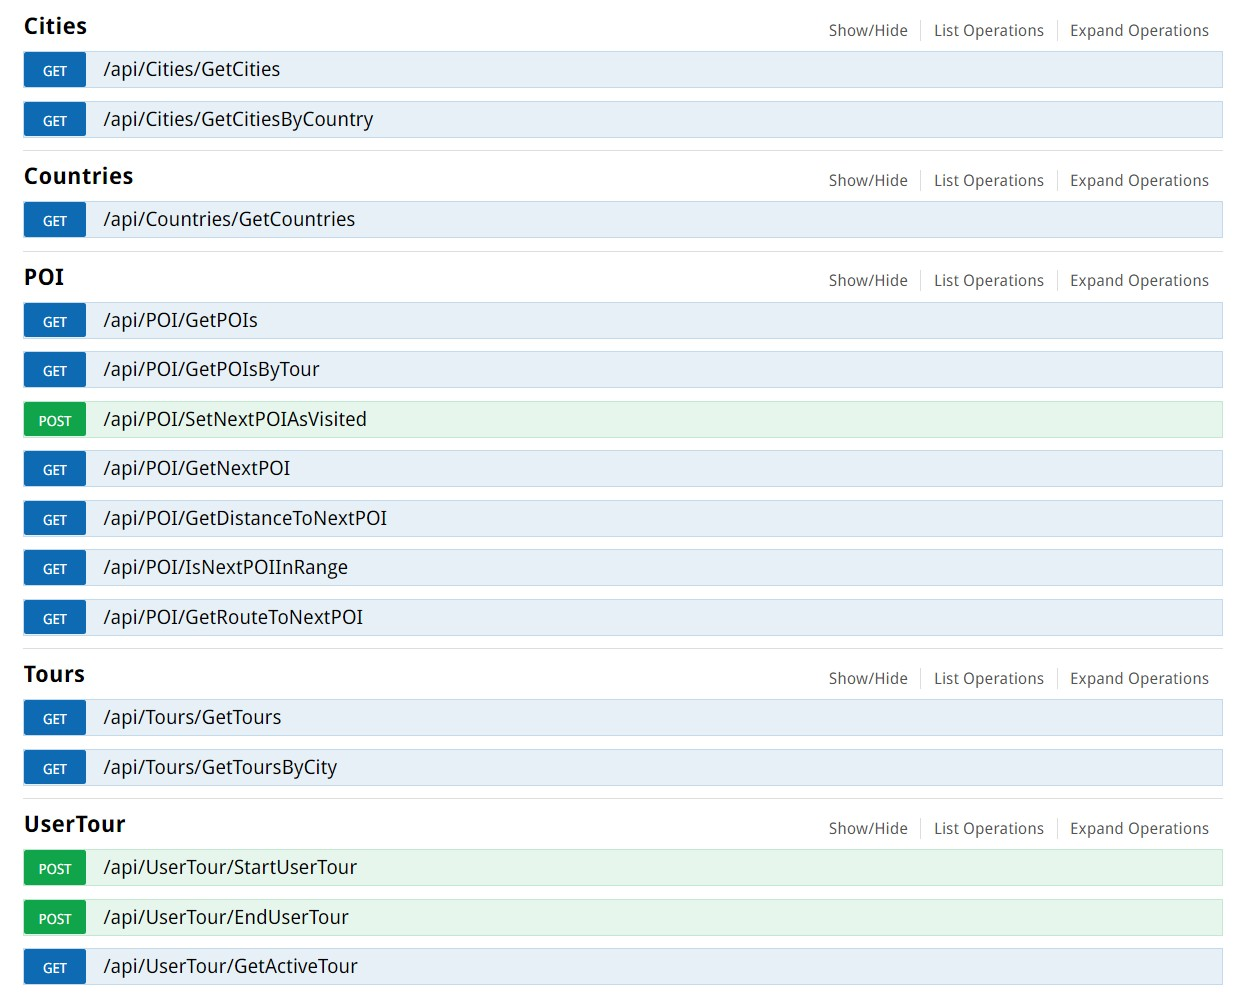
\includegraphics{swagger_schlussbericht}
  \caption{Übersicht API}
\end{figure}

Controller:

\begin{longtabu} to \textwidth { | l | X[l] | }
\hline
\textbf{Controller} & \textbf{Beschreibung} \\
\hline
\endhead

Cities & Implementiert alle Funktionalit\"aten zum Abfragen und \"Andern von
  St\"adte-Daten\\ \hline
Countries & Implementiert alle Funktionalit\"aten zum Abfragen und \"Andern von
  L\"ander-Daten\\ \hline
POI & Implementiert alle Funktionalit\"aten zum Abfragen und \"Andern von Point of
Interests, welche durch eine Tour verkn\"upft sind. Zudem alle Funktionalit\"aten zum Abfragen und \"Andern von UserPOIs.
  Ein User POI ist ein Point of Interest welcher von einem Benutzer besucht wurde oder
  welcher ein Benutzer im Rahmen seiner gestarteten Tour als n\"achstes besuchen muss.\\\hline
Tours & Implementiert alle Funktionalit\"aten zum Abfragen und \"Andern von Touren. Zudem alle Funktionalit\"aten zum Abfragen und \"Andern von UserTouren.
  Eine UserTour ist eine Tour die von einem Benutzer gestartet wurde.\\\hline
\end{longtabu}

Die API wurde gegenüber dem Design-Entwurf vereinfacht, vereinheitlicht und die Unterscheidungslogik zwischen z.B. POI und UserPOI wurde nach aussen weggekapselt.
Nicht mehr vorhandene Methoden in der aktuellen Version sind mit removed gekennzeichnet.

Methoden:

\begin{longtabu} to \textwidth { | l | X[l] | }
\hline
\textbf{Methode} & \textbf{Beschreibung} \\
\hline
\endhead

api/Cities/GetCities &
Liefert eine Liste aller vorhandenen St\"adte.\\\hline
api/Cities/GetCitiesByCountry &
Liefert eine Liste aller vorhandenen St\"adte in einem bestimmten Land.\\\hline
  api/Countries/GetCountries &
Liefert eine Liste aller vorhandenen L\"ander.\\\hline
api/POI/GetPOIs &
Liefert eine Liste aller vorhandenen POIs.\\\hline
api/POI/GetPOIsByTour &
Liefert eine Liste aller POIs zu einer bestimmten Tour.\\\hline
api/POI/SetNextPOIAsVisited &
Markiert den n\"achsten POI, den ein bestimmter Benutzer aufgrund seiner aktiv gestarteten
  Tour besuchen muss, als besucht.\\\hline
  api/POI/GetNextPOI &
Liefert f\"ur eine Benutzer-ID den n\"achsten POI zur\"uck, den der Benutzer besuchen
  muss.\\\hline
  api/POI/GetDistanceToNextPOI &
Gibt aufgrund von Geokoordinaten und einer Benutzer-ID die Distanz bis zu einem n\"achsten POI
  den der Benutzer mit seiner gestarteten Tour besuchen muss.\\\hline
api/POI/IsNextPOIInRange &
Gibt aufgrund von Geokoordinaten und einer Benutzer-ID zur\"uck, ob die Koordinaten gen\"ugend
  nahe am n\"achsten POI, den der Benutzer mit seiner gestarteten Tour besuchen muss, ist.

Die erlaubte Distanz kann als optionaler Parameter mitgegeben werden.\\\hline
  api/POI/GetRouteToNextPOI &
Liefert aufgrund einer Benutzer-ID die Route als einzelne Navigationspunkte zum n\"achsten
  POI, den der Benutzer mit seiner gestarteten Tour besuchen muss.\\\hline
api/POI/GetDistanceToPOI (removed) &
Gibt aufgrund von Geokoordinaten die Distanz bis zu einem bestimmten POI zur\"uck.\\\hline
api/POI/IsPOIInRange (removed)&
Gibt aufgrund von Geokoordinaten zur\"uck, ob diese gen\"ugend nahe an einem POI sind. Die
  erlaubte Distanz kann als optionaler Parameter mitgegeben werden. \\\hline
api/UserPOI/CheckUserTourPOI (removed) &
Markiert einen bestimmten POI in einer UserTour als besucht.\\\hline
api/UserPOI/CheckPOI (removed) &
  Markiert einen bestimmten POI f\"ur eine angegebene Tour und eine definierte Benutzer-ID als
  besucht.\\\hline
api/Tours/GetTours &
Gibt alle vorhandenen Touren zur\"uck.\\\hline
api/Tours/GetToursByCity &
Gibt alle vorhanden Touren in einer bestimmten Stadt zur\"uck.\\\hline
api/UserTour/StartUserTour &
Startet eine definierte Tour f\"ur einen bestimmten Benutzer. Liefert direkt eine Auflistung
  aller POIs und Routenpunkte dieser Tour zur\"uck.\\\hline
api/UserTour/EndUserTour &
Beendet die aktive UserTour f\"ur einen bestimmten Benutzer. \\\hline
api/UserTour/GetActiveTour &
Gibt die aktive Tour des Benutzers zur\"uck.\\\hline
\end{longtabu}

\subsubsubsection{Versionierung der API}\label{versionierung-api}
F\"ur gr\"ossere \"Anderungen an der API soll aus Kompatibilit\"atsgr\"unden eine neue Version erstellt und parallel zu
\"alteren Versionen deployt werden. Swashbuckle bietet auch hierf\"ur die notwendige Funktionalit\"at zur Versionierung
an.

\subsubsection{Externe Frameworks}\label{externe-frameworks}
Zur Implementierung von architektonischen und business-funktionalen Anforderungen, die nicht bereits mit ASP.NET MVC und
Web API abgedeckt sind, sollen bereits bestehende Libraries und Frameworks verwendet werden. Die nachfolgende Tabelle
listet die zu verwenden Frameworks auf:

\begin{longtabu} to \textwidth { | l | l | l | X[l] | }
\hline
\textbf{Framework} & \textbf{Version}  & \textbf{Typ} & \textbf{Beschreibung} \\
\hline
\endhead

Google Maps API &
0.65 &
Funktional &
Wird verwendet um die funktionalen Anforderungen wie Routenberechnung usw. zu
  implementieren.\\\hline
Ninject &
3.2.0 &
Architektur &
Ninject ist ein Dependency Injection Framework, welches eine Integration f\"ur ASP.NET
  anbietet. Mit Dependency Injection sollen die einzelnen Repositories den Controllern zur Verf\"ugung gestellt werden.
  Dadurch soll ebenfalls gew\"ahrleistet werden, dass pro Request und Repository nur genau eine Datenbankverbindung
  aufgebaut und dann auch wieder sauber geschlossen wird. So werden Performance- und Datenkonsistenzprobleme, sowie
  Probleme mit nicht geschlossenen Datenbankverbindungen vermieden.\\\hline
Swashbuckle &
5.2.1 &
Architektur &
Swashbuckle erm\"oglicht das automatische Generieren und Anzeigen von Swagger Interface
  Descriptions zur Laufzeit. Mit Hilfe dieser Descriptions k\"onnen die Services einfacher integriert werden, indem zum
  Beispiel die Datenobjekte oder Proxy-Klassen auf Konsumentenseite automatisch generiert werden k\"onnen.\\\hline
Log4Net &
2.0.8 &
Nicht-Funktional &
Framework zum Loggen von Fehlern, Warnungen und Debug-Informationen an verschiedene
  Appenders wie Datenbank oder Logfile.\\\hline
\end{longtabu}


\subsubsection{Architektur}\label{backendarchitektur}
Das nachfolgende Diagramm zeigt die Detail-Architektur des Backends. Weitere grundlegende
Informationen zum eingesetzten Technologie-Stack befinden sich im Dokument Anforderungsanalyse.

\begin{figure}
  \centering
  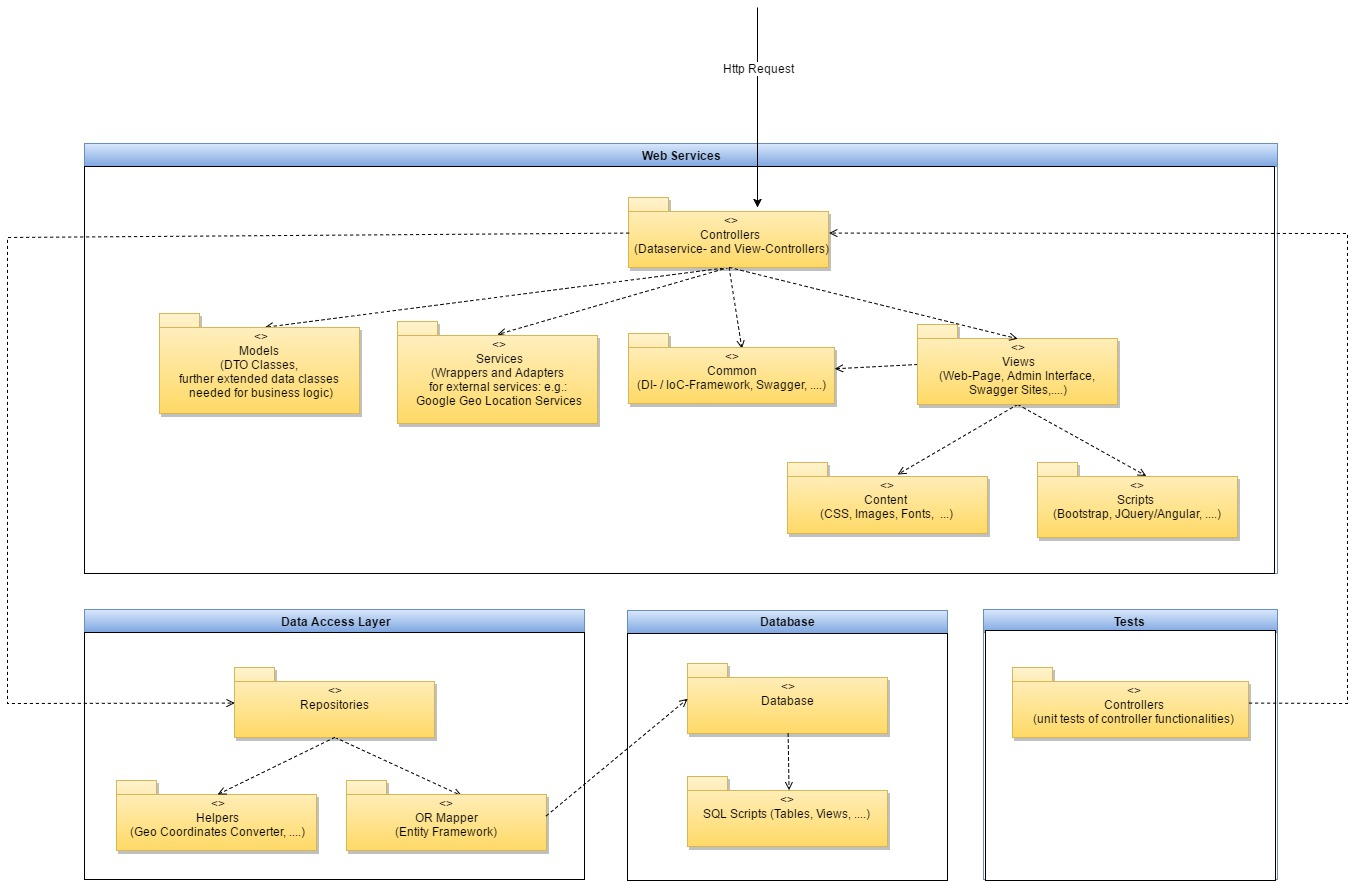
\includegraphics{backend_architektur_schlussbericht}
  \caption{Backend Architektur}
\end{figure}

\newpage
\begin{longtabu} to \textwidth { | l | l | X[l] | }
\hline
\textbf{Layer} & \textbf{Package}  & \textbf{Beschreibung} \\
\hline
\endhead

Web Services &
Controllers &
Controllers beinhaltet alle WebAPI- sowie MVC-Controller, welche die ankommenden Requests
  bearbeiten.

Ein Controller hat mindestens eine Methode und wird \"uber eine spezifische Sub-Url
  aufgerufen. ASP.NET WebAPI/MVC \"ubernimmt das automatische Mapping des ankommenden Requests mit den entsprechenden
  Parametern inkl. Request-Type \ und findet die passende Methode des Controllers, die diesen Request verarbeiten kann.
  Ein API Controller liefert nur Daten in JSON oder XML Format und keine darstellungsspezifischen Informationen.

Zu einem sp\"ateren Zeitpunkt k\"onnen f\"ur die Implementierung der Web-Applikation als
  Administrations-Interface MVC-Controller erstellt werden welche eine entsprechende HTML View zur\"uckgeben. S\"amtliche
  Daten sollen aber auch hier dynamisch \"uber API-Controller mit AJAX-Requests geladen werden. Es sollen keine Seiten
  mit Daten serverseitig gerendert werden.\\\hline
Web Services &
Models &
Dieses Paket beinhaltet alle Model-Klassen welche in den Webservices ben\"otigt werden. Diese
  Klassen unterscheiden sich durch Attribut-Erg\"anzungen (z.B. f\"ur aggregierte oder aufgeschl\"usselte Datenfelder)
  gegen\"uber den vom Entity-Framework generierten Datenklassen welche prim\"ar die Datenbankstruktur abbilden.

Hier befindet sich auch die Funktionalit\"at zum Mappen der Entity-Framework-Datenklassen auf
  DTO Klassen.\\\hline
Web Services &
Services &
Hier sind alle Adapter- und Wrapperklassen f\"ur externe Service angesiedelt, welche f\"ur
  weitere Funktionalit\"aten vom Backend aufgerufen werden.\\\hline
Web Services &
Common &
Dies beinhaltet alle Klassen und Funktionalit\"aten welche \"uber das ganze Projekt hinweg
  ben\"otigt werden. Hierbei handelt es sich zum Beispiel um die ganze Dependency Injection oder Swagger
  Funktionalit\"at.\\\hline
Web Services &
Views &
Zu einem sp\"ateren Zeitpunkt soll neben den Datenservices auch eine Webapplikation erstellt
  werden, welche das Administrieren der Daten erm\"oglichen soll. Hierf\"ur k\"onnen in diesem Package HTML Views
  erstellt werden.\\\hline
Web Services &
Content &
Content beinhaltet den Content der f\"ur die Darstellung der Views ben\"otigt wird wie zum
  Beispiel CSS-Files, Bilder, Fonts usw.\\\hline
Web Services &
Scripts &
Hier werden alle Skripts abgelegt die client-seitig ben\"otigt werden. Es handelt sich hierbei
  vor allem um selbst erstellte Javascript-Funktionalit\"aten und Javascript Frameworks wie JQuery, Angular, Bootstrap
  usw. Die Details zur Implementierung des Webinterfaces werden zu einem sp\"ateren Zeitpunkt genauer definiert.\\\hline
Data Access Layer &
Repositories &
Grunds\"atzlich existiert f\"ur jede Datenklasse aus der Datenbank ein Repository, welche die
  Daten (teil-)aggregiert und funktional zur Verf\"ugung stellt. Dadurch ist die Wiederverwendbarkeit grundlegender oder
  kombinierter Datenabfragen gew\"ahrleistet.\\\hline
Data Access Layer &
Helpers &
Zum Beispiel f\"ur das Umwandeln der Koordinaten-Angaben vom MSSQL-Format in einzelne
  Werteangaben f\"ur L\"angen- und Breitengrade werden Helferklassen ben\"otigt, welche hier angesiedelt sind.\\\hline
Data Access Layer &
OR Mapper &
Als klassischer OR Mapper wird das Entity Framework mit dem Database First Vorgehen verwendet.
  Dies bedeutet, dass basierend auf der Datenbank automatisch Proxy-Datenklassen vom Entity-Framework generiert
  werden.\\\hline
Database &
Database &
Das Datenbankprojekt wird vollst\"andig als MSSQL Datenbank Projekt umgesetzt. Damit werden
  automatisch \"Anderungen an den SQL Dateien im Projekt getrackt und es k\"onnen unter Beachtung dieser \"Anderungen
  automatisch Datenbank Installations-Packages (DACPAC) generiert werden, welche den initialen Stand oder ein Delta
  beinhalten.\\\hline
Database &
SQL Scripts &
Die eigentlichen SQL Skripts f\"ur Tables, Views oder weitere Datenbank-Elemente.\\\hline
Tests &
Controllers &
Dieses Testprojekt implementiert alle Unit-Tests zum automatischen Testen der WebAPI
  Controller-Funktionalit\"aten. \\\hline
\end{longtabu}

\subsubsubsection{Ablauf eines Request und Datenfluss aus technischer Sicht}\label{ablauf-request}
Der nachfolgende Prozess zeigt den programmatischen Standardablauf eines Request im Backend, inklusive dem Datenfluss
von der Datenbank bis zum Inhalt in der HTTP-Response, auf:

\begin{enumerate}
  \item
    Der Controller erh\"alt einen Request. Bei der Instanzierung des Controller werden automatisch \"uber Dependency Injection
    die ben\"otigten Repositories instanziert und mitgegeben. Ein Repository erstellt bei der Instanzierung automatisch
    eine Datenbankverbindung. F\"ur einen Request wird so pro Repository nur eine einzige Datenbankverbindung aufgebaut, da
    auch nur eine Repository-Instanz erstellt wird.
  \item
    Die Repository-Klasse extrahiert die ben\"otigten Daten mit LINQ-Queries und gibt diese immer als IQueryable
    R\"uckgabewert zur\"uck. Damit lassen sich einzelne Repository-Abfragen theoretisch auch hintereinanderschalten oder es
    sind weitere Operationen auf dem Datensatz m\"oglich.
  \item
    Die Daten werden \"uber das Datenmodel vom Entity-Framework beim Materialisieren des LINQ-Queries geladen.
  \item
    Die Controller-Funktion erstellt eine Instanz des DTO. Dies geschieht entweder mit automatischen Mapping \"uber
    Reflection f\"ur gleiche Felder wie die Datenklassen des Entity Framework Modells oder falls ben\"otigt mit manuellen
    Mapping \"uber eine wiederverwendbare Lambda Function Expression f\"ur einzelne oder mehrere Properties. Diese kann
    direkt auf das erhaltene IQueryable als Select-Befehl angewendet werden.
  \item
    Der Controller gibt das Resultat zusammen mit einem Statuscode zur\"uck.
  \item
    Die Repository Instanz wird nicht mehr ben\"otigt. Die Datenbankverbindung wird geschlossen und die Instanz disposed.
\end{enumerate}

\newpage
\subsubsubsection{Dependency Injection}\label{dependency-injection}
Als Dependency Injection Framework f\"ur die Umsetzung des Inversion of Control Patterns wird Ninject eingesetzt.
Ninject bietet eine statische Konfiguration zum Binden von Interfaces an bestimmte Klassen welche bei einer solchen
Anfrage instanziert werden m\"ussen. Eine solche Implementierung bietet eine bessere Performance als wenn die zu
instanziierenden Klassen im ganzen Projekt zuerst gesucht werden m\"ussen. Die Services welche injected werden, sollen
als One-Per-Request Modul definiert sein.


Da ein Controller von der erfolgreichen Instanzierung seines ben\"otigten Repositories abh\"angig ist (strong-coupled),
w\"are in einer n\"achsten Version eine Implementierung der Repositories als Lazy-Object sinnvoll. Dadurch w\"urde die
Instanzierung erst beim ersten Zugriff innerhalb des Controllers geschehen und es k\"onnte bei einem Problem spezifisch
darauf reagiert werden. Bei der direkten Injection ist dies nur begrenzt m\"oglich, da dann entweder vorher einen Fehler
geworfen wird oder aber die injezierten Parameter als Null daherkommen.

\subsubsubsection{Logging}\label{logging}
Das Logging wird mit Hilfe der Log4Net Library implementiert. Geloggt werden soll in t\"agliche Rolling-Logfiles, was
als Appender in Log4Net konfiguriert werden kann.

\subsubsubsection{Security}\label{security}
Das Thema Security inklusive Authentifizierung und Authentisierung von Benutzern, die Implementierung von verschiedenen
Rollen, das Verschl\"usseln der Kommunikation usw. soll f\"ur die erste Version des Backends nicht beachtet werden.

\subsubsubsection{Testing}\label{testing}
F\"ur die Implementierung von Unit-Tests der Controller, muss ein Controller manuell instanziert werden k\"onnen. Dies
bedeutet, dass jede Controller-Klasse einen leeren Konstruktor implementieren muss, in welchem die ben\"otigten
Repositories manuell instanziert werden.

\subsubsubsection{Swagger}\label{swagger}
\"Uber Swashbuckle wird die automatische Generierung von Swagger Interface Definitions implementiert.

\begin{longtabu} to \textwidth { | X[l] | X[l] | }
\hline
\textbf{Url} & \textbf{Content} \\\hline
\endhead

\url{http://travelbuddy5.azurewebsites.net/swagger/ui/index} & Url zum Aufruf der
  generierten Seite inklusive Methoden zum direkten, parametrisierten Aufruf.\\\hline
\url{http://travelbuddy5.azurewebsites.net/swagger/docs/v1} & Url zum Aufruf der generierten
  JSON Interface Definition. Die Versionsnummer kann je nach Version der API angegeben werden.\\\hline
\end{longtabu}

\newpage
\subsubsection{Klassendiagramme und Klassenverantwortlichkeiten}\label{klassendiagramme}
Dieses Diagramm zeigt das Zusammenspiel der Controller mit den jeweiligen Repositories.

\begin{figure}
  \centering
  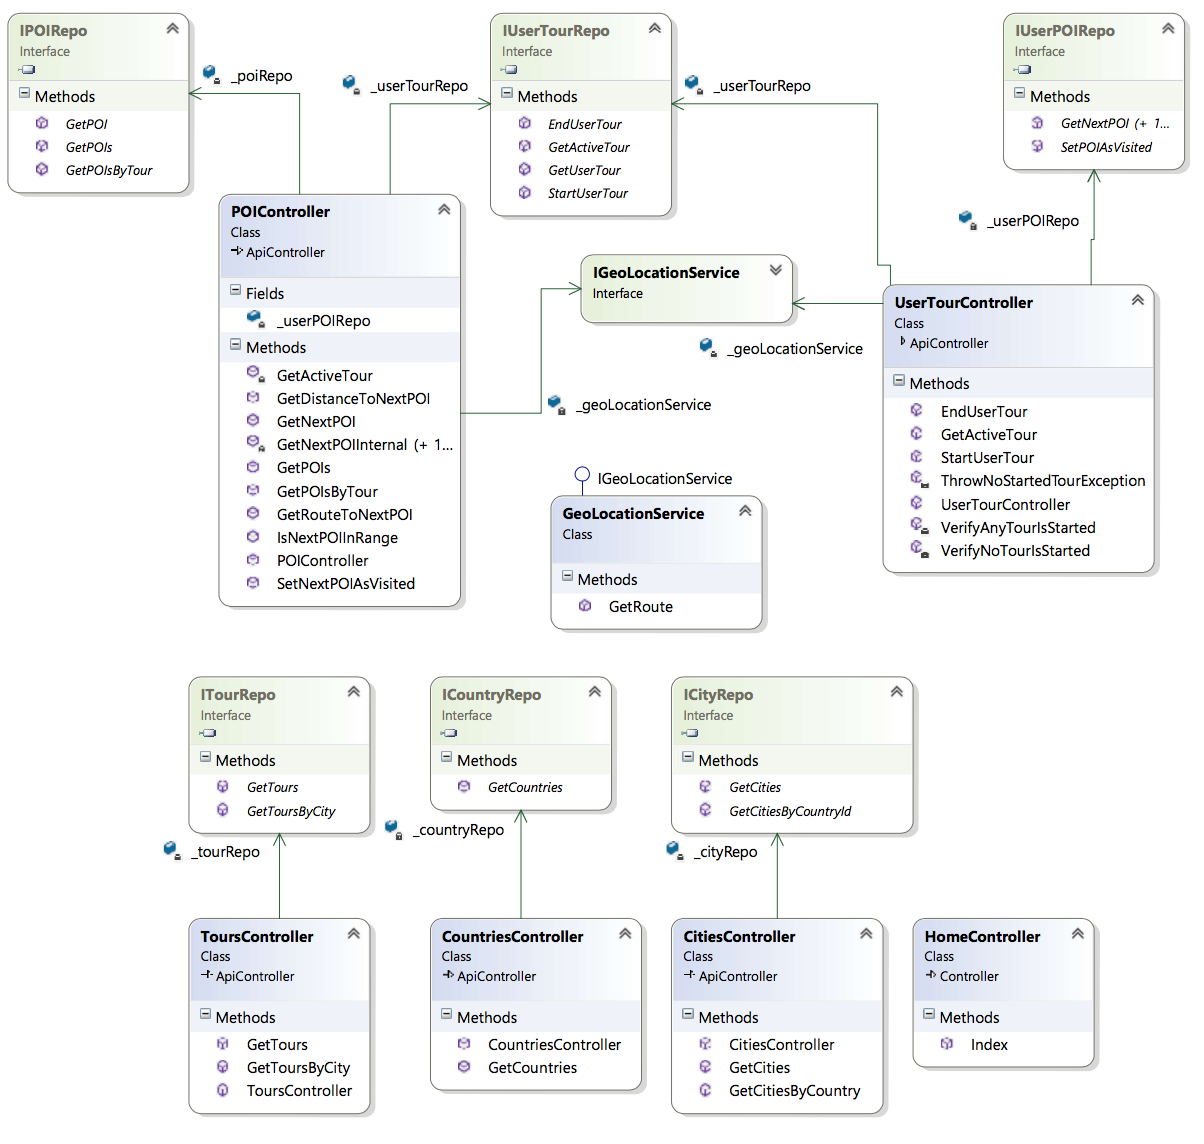
\includegraphics{klassendiagramm_backend_schlussbericht1}
  \caption{Klassendiagramm mit Zusammenspiel der Controller und den jeweiligen Repositories}
\end{figure}

Die Controller weisen die in der Service API beschriebenen Funktionalit\"aten und Verantwortlichkeiten auf. Sie
behandeln alle ankommenden Requests und verwenden daf\"ur 1-n Repositories (da es sich nicht um reine CRUD Controller
handelt, k\"onnen auch mehrere Repositories verwendet werden) um die Daten aus der Datenbank zu holen und beliebige
Services, wie zum Beispiel den GeoLocationService, welcher einen Wrapper f\"ur die Google Maps Geo Location Services
implementiert. Services und Repositories werden wie bereits beschrieben \"uber Dependency Injection den Controllern zur
Verf\"ugung gestellt. Der HomeController dient als Einstiegspunkt der WebApplikation und ist daher kein API Controller.
Er liefert eine HTML View zur\"uck.

Die DTO Klassen sind erweiterte Datenklassen basierend (aber nicht vererbt) auf den vom Entity-Framework automatisch
generierten Datenklassen. Dies erm\"oglicht eine Erg\"anzung der Attribute um aggregierte oder separierte Werte.

\begin{figure}
  \centering
  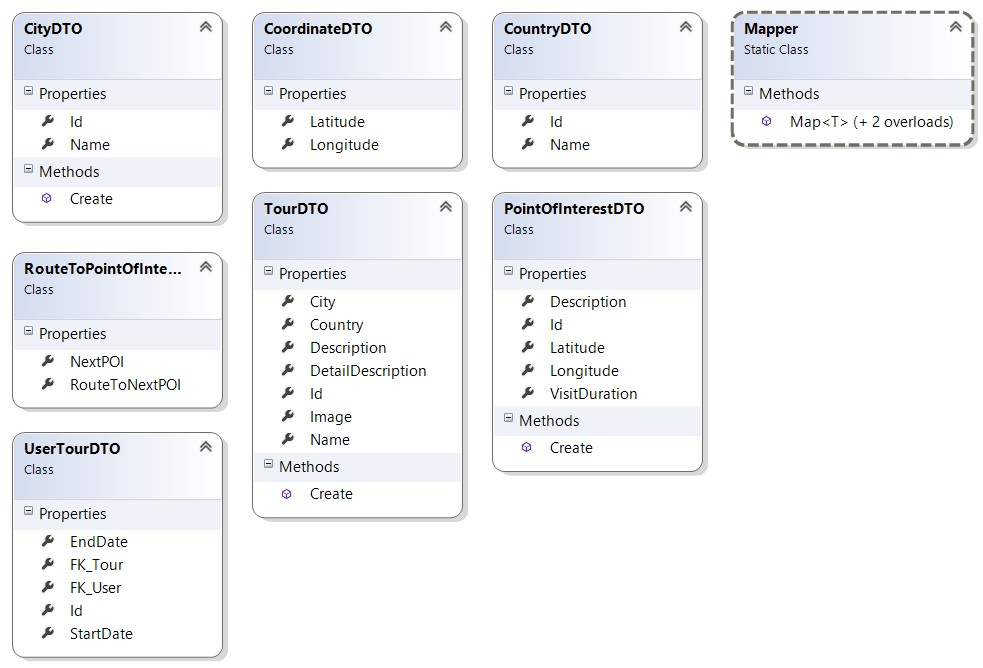
\includegraphics{klassendiagramm_backend_schlussbericht2}
  \caption{Klassendiagramm DTO Klassen}
\end{figure}

Hier speziell zu erw\"ahnen sind die statische Mapper Klasse und der wiederverwendbare POIMapper. Die generische Mapper
Klasse mappt mit Hilfe von Reflection eine Datenklasse des Entity-Frameworks direkt auf gleichnamige Felder der
gew\"unschten DTO Klasse. Diese Funktionalit\"at kann f\"ur alle Felder verwendet werden die eins zu eins in beiden
Datenklassen vorhanden sind und den gleichen Datentypen besitzen. Ein manuelles Mappen dieser Felder ist damit nicht
mehr notwendig. Die DTO Klassen stellen die manuelle Mapping-Logik z.B. f\"ur das Aufsplitten der Geo-Koordinaten in
Latitude und Longitude in wiederverwendbarer Form bereit. Sie liefern eine LINQ Function-Expression zur\"uck, welche die
Mapping-Logik definiert.

\newpage
Die Repository Klassen implementieren das jeweilige von den Controllern von aussen her verwendete Interface.

\begin{figure}
  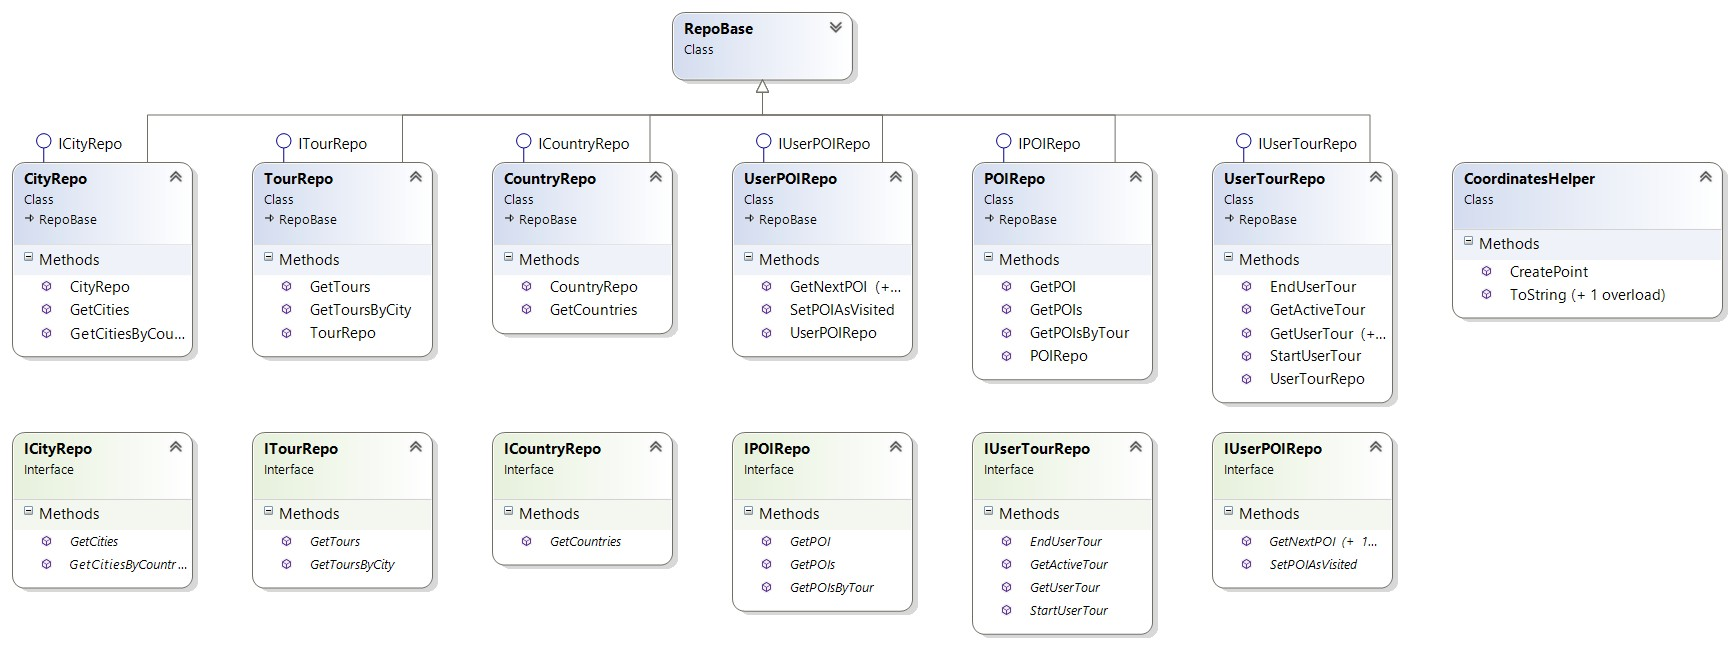
\includegraphics{klassendiagramm_backend_schlussbericht3}
  \caption{Klassendiagramm der Repository Klassen}
\end{figure}

Die einzelnen Repositories implementieren den Zugriff \"uber LINQ-Queries auf die vom Vorbild der Datenbank generierten
Datenklassen\--Objekte. Sie sind alle von der Klasse RepoBase abgeleitet. RepoBase \"offnet bei der Instanzierung
automatisch eine Datenbankverbindung und stellt diese Verbindung den abgeleiteten Klassen zur Verf\"ugung. Die fachlichen und
funktionalen Verantwortlichkeiten werden analog zu den Zust\"andigkeiten der Controller implementiert. Im Kapitel
Service API werden daf\"ur die notwendigen Begriffe und Unterteilungen detailliert erl\"autert.

Speziell ist hier die Klasse CoordinatesHelper.
Der CoordinatesHelper \"ubersetzt das MSSQL Datenbankformat der Geo-Koordinaten in einzelne ben\"otigte Werte wie
L\"angen- und Breitengrad und umgekehrt.

\newpage
\subsubsection{Entity Relationship Diagram}\label{erm}
Als Erg\"anzung und zum besseren Verst\"andnis der Zusammenh\"ange nachfolgend das Diagramm des Datenbankmodels.

\begin{figure}
  \centering
  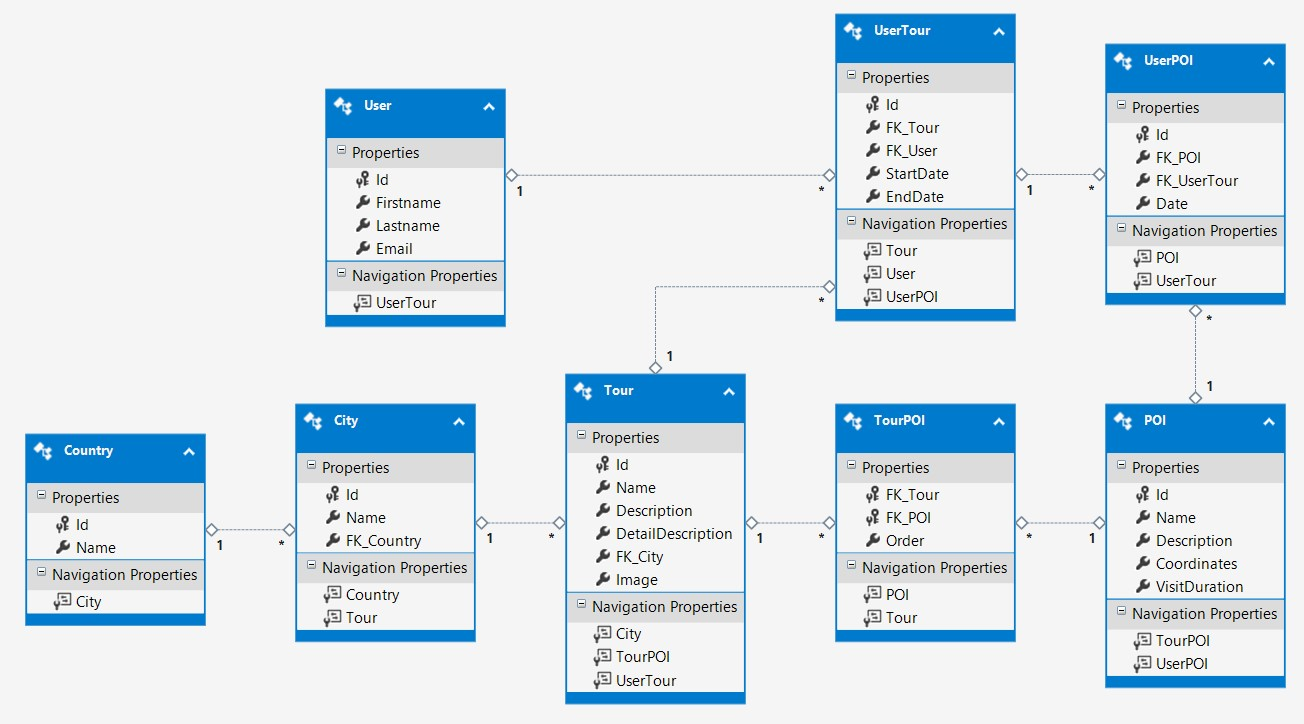
\includegraphics{erm_schlussbericht}
  \caption{Entity Relationship Diagram}
\end{figure}
